%!TEX root = ../../beamer.tex
\begin{frame}
\frametitle{stochasticity in gene expression}
\begin{center}
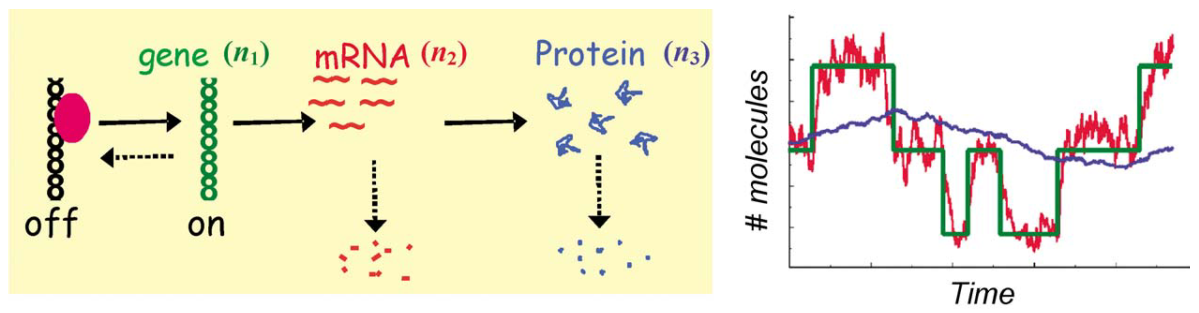
\includegraphics[width=0.9\textwidth]{fig/stochgeneexpdyn.png}\\

{\scriptsize
$n_1$ number of active genes, $n_2$ number of mRNAs, $n_3$ proteins per cell
\begin{align*}
\text{gene activation } &n_1 \xrightarrow{\lambda_1^+ (n_1^{max}-n_1)}n_1+1\\
\text{gene inactivation } &n_1 \xrightarrow{\lambda_1^- n_1}n_1-1\\
\text{transcription } &n_2 \xrightarrow{\lambda_2 n_1}n_2+1\\
\text{mRNA degradation } &n_2 \xrightarrow{n_2/\tau_2}n_2-1\\
\text{translation } &n_3 \xrightarrow{\lambda_3 n_2}n_3+1\\
\text{proteolysis } &n_3 \xrightarrow{n_3/\tau_3}n_3-1
\end{align*}}
\end{center}
\hfill \cite{Paulsson2005}
\end{frame}

